\begingroup\small
\begin{longtable}{>{\raggedright\arraybackslash}p{.16\linewidth}>{\raggedright\arraybackslash}p{.52\linewidth}>{\raggedright\arraybackslash}p{.27\linewidth}}
\caption{네 유형과 별도 IDS 참고 연구의 구조 비교. 각 방법의 원문 대표 그림을 아래 개별 설명에서 확대 제시한다. 그림의 출처·페이지는 보관 PDF 기준이다.}\\
\toprule 방법·계열 & 원문 대표 그림 & 학습·배포 방식과 우리 설계의 차이\\\midrule\endfirsthead
\toprule 방법·계열 & 원문 대표 그림 & 학습·배포 방식과 우리 설계의 차이\\\midrule\endhead
\bottomrule\endfoot
\rowcolor{blue!12}
\multicolumn{3}{l}{\textbf{유형 1: 사전학습·가중치 적응}}\\*
\rowcolor{blue!4}
\textbf{TabDPT}\par\footnotesize (NeurIPS, 2025): 실제 표 사전학습 &
\begin{minipage}[t]{\linewidth}\vspace{0pt}\centering
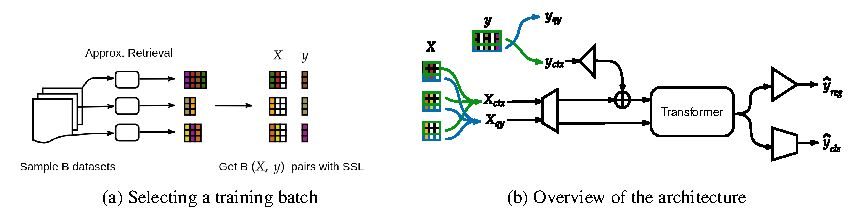
\includegraphics[width=\linewidth,height=4.1cm,keepaspectratio]{figures/20261028_design_sota/tabdpt.pdf}
\par\scriptsize\href{https://arxiv.org/pdf/2410.18164}{Figure 2 · PDF 5쪽 / 원문}\end{minipage} &
실제 표의 열 예측 과제로 기반 모델을 학습했다. 1안은 범용 기반 모델 재학습 대신 별도 학생을 적응시킨다. 비라벨 접근 조건을 맞춘다.\\[7pt]\midrule
\textbf{LoCalPFN}\par\footnotesize (NeurIPS, 2024): 검색 + 가중치 적응 &
\begin{minipage}[t]{\linewidth}\vspace{0pt}\centering
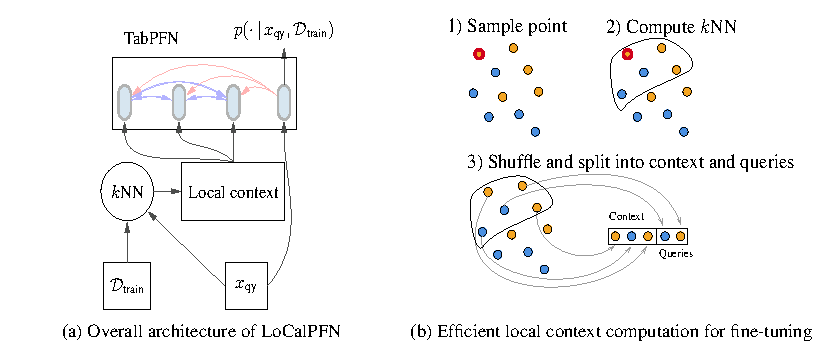
\includegraphics[width=\linewidth,height=4.1cm,keepaspectratio]{figures/20261028_design_sota/local.pdf}
\par\scriptsize\href{https://papers.nips.cc/paper_files/paper/2024/file/c40daf14d7a6469e65116507c21faeb7-Paper-Conference.pdf}{Figure 3 · PDF 5쪽 / 원문}\end{minipage} &
근접 context 검색과 PFN fine-tuning을 결합했다. 2안의 이진 쌍 분리는 query별 검색이 아니며 PFN 가중치를 고정한다.\\[7pt]\midrule
\rowcolor{blue!12}
\multicolumn{3}{l}{\textbf{유형 2: 앙상블}}\\*
\rowcolor{blue!4}
\textbf{BoostPFN}\par\footnotesize (AISTATS, 2025): 순차 앙상블 &
\begin{minipage}[t]{\linewidth}\vspace{0pt}\centering
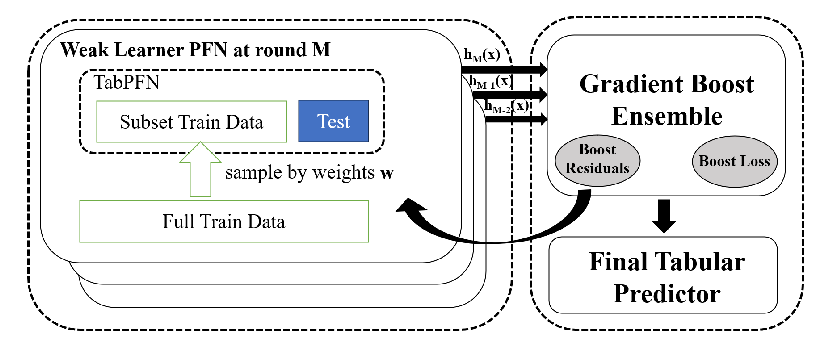
\includegraphics[width=\linewidth,height=4.1cm,keepaspectratio]{figures/20261028_design_sota/boost.pdf}
\par\scriptsize\href{https://arxiv.org/pdf/2503.01256}{Figure 1 · PDF 2쪽 / 원문}\end{minipage} &
잔차로 다음 context를 선택하고 예측기를 더했다. 2안은 전체 클래스 출력을 더하는 대신 선택한 두 logit의 차이를 제한 수정한다.\\[7pt]\midrule
\textbf{BETA}\par\footnotesize (ICML, 2025): encoder + 앙상블 &
\begin{minipage}[t]{\linewidth}\vspace{0pt}\centering
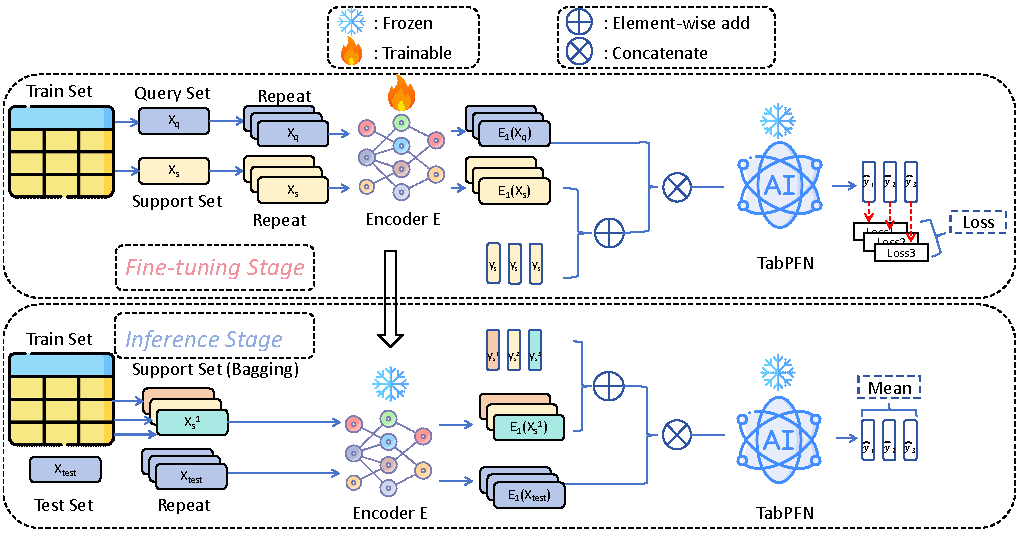
\includegraphics[width=\linewidth,height=4.1cm,keepaspectratio]{figures/20261028_design_sota/beta.pdf}
\par\scriptsize\href{https://arxiv.org/pdf/2502.02527}{Figure 3 · PDF 6쪽 / 원문}\end{minipage} &
PFN은 고정하고 입력 encoder를 학습했다. 여러 표현과 bootstrap context의 PFN 예측을 평균했다. 1안의 학생 단독 배포·2안의 쌍 수정과 구별한다.\\[7pt]\midrule
\rowcolor{blue!12}
\multicolumn{3}{l}{\textbf{유형 3: 출력 확률 보정}}\\*
\rowcolor{blue!4}
\textbf{DistPFN}\par\footnotesize (ICML, 2026): posterior 보정 &
\begin{minipage}[t]{\linewidth}\vspace{0pt}\centering
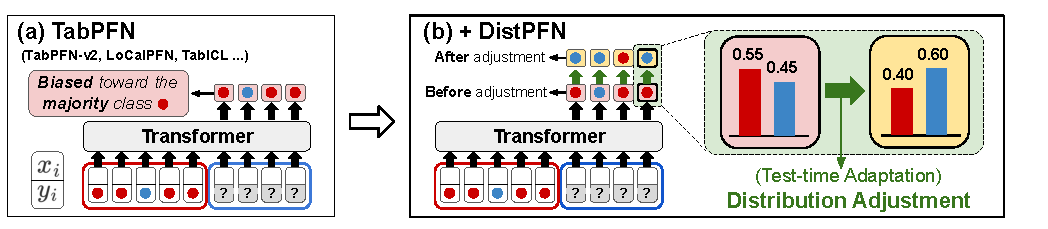
\includegraphics[width=\linewidth,height=4.1cm,keepaspectratio]{figures/20261028_design_sota/dist.pdf}
\par\scriptsize\href{https://arxiv.org/pdf/2605.04363}{Figure 4 · PDF 4쪽 / 원문}\end{minipage} &
가중치 학습 없이 context prior와 예측 posterior로 보정했다. 쌍 경계 학습과 별도 요소이며 query 집합 통계 접근을 공개한다.\\[7pt]\midrule
\rowcolor{blue!12}
\multicolumn{3}{l}{\textbf{유형 4: context 관리}}\\*
\textbf{CURE}\par\footnotesize (FMSD@ICML Workshop, 2026): 고정 용량 버퍼 &
\begin{minipage}[t]{\linewidth}\vspace{0pt}\centering
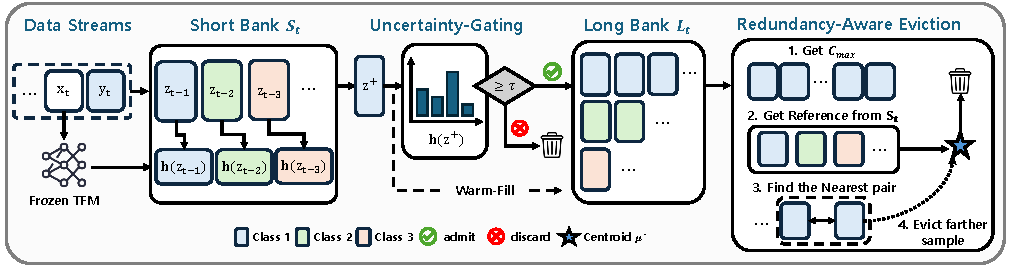
\includegraphics[width=\linewidth,height=4.1cm,keepaspectratio]{figures/20261028_design_sota/cure.pdf}
\par\scriptsize\href{https://arxiv.org/pdf/2606.18677}{Figure 1 · PDF 3쪽 / 원문}\end{minipage} &
최근 short bank와 불확실성·중복 기준 long bank를 갱신했다. 고정한 것은 용량이며 내용은 바뀐다. 기존 EXP84 버퍼 정책과 직접 비교할 대상이다.\\[7pt]\midrule
\rowcolor{blue!12}
\multicolumn{3}{l}{\textbf{별도 IDS 참고 연구: TabPFN 계열 외 접근}}\\*
\rowcolor{blue!4}
\textbf{LotBoNC}\par\footnotesize (AsiaCCS, 2026): 표현·대표점 학습 &
\begin{minipage}[t]{\linewidth}\vspace{0pt}\centering
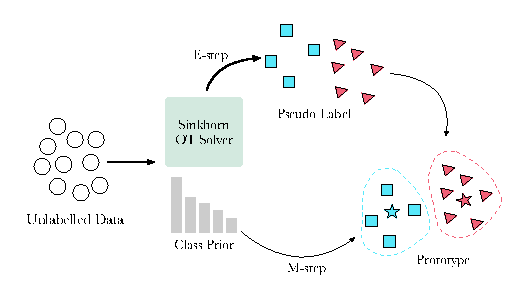
\includegraphics[width=\linewidth,height=4.1cm,keepaspectratio]{figures/20261028_design_sota/lotbonc.pdf}
\par\scriptsize\href{https://doi.org/10.1145/3779208.3785276}{Figure 4 · PDF 5쪽 / 원문}\end{minipage} &
바이트 encoder와 대표점을 갱신했다. 비균등 soft 배정이 핵심이다. 1안은 수치 flow와 TabPFN 교사를 추가하며 학생을 배포한다.\\[7pt]\midrule
\end{longtable}
\endgroup
